\chapter{Ajuster un modèle de régression linéaire multiple (RLM)}
\label{sec:AjusterRLM}

% À voir la pertinence de cette section
\vspace{-0.1in}
\section{Préambule : notation matricielle de la RLS}

Le traitement de la régression linéaire peut être grandement approfondi
en utilisant la notation matricielle et les résultats de l'algèbre linéaire. On considère d'abord la notation matricielle dans le cas de la régression linéaire simple, i.e. avec une seule variable explicative.

Soient $\boY$, le vecteur de dimension $(n\times 1)$ des observations de la variable endogène, $\boX$ la matrice de dimension $(n\times 2)$ des valeurs de la variable exogène, $\bobeta$ le vecteur de dimension $(2\times 1)$ des coefficients de régression et $\boeps$ le vecteur de dimension $(n \times 1)$ des termes d'erreurs:
$$
\boY=\underbrace{\left(\begin{array}{c} Y_1\\ Y_2\\ \vdots\\ Y_n\end{array}\right)}_{n\times 1}
\ \ \ \bobeta=\underbrace{\left({\beta_0\atop\beta_1}\right)}_{2 \times 1}\ \ \
\boX=\underbrace{\left(\begin{array}{cc} 1 & x_1\\ 1 & x_2\\ \vdots & \vdots \\
1 & x_n\end{array}\right)}_{n\times 2}\ \ \
\boeps=\underbrace{\left(\begin{array}{c}\varepsilon_1\\ \varepsilon_2\\ \vdots\\
\varepsilon_n\end{array}\right)}_{n\times 1}.
$$
On a que
$$\underbrace{\left(\begin{array}{c} Y_1\\ Y_2\\ \vdots\\ Y_n\end{array}\right)}_{n\times 1}=\underbrace{\left(\begin{array}{cc} 1 & x_1\\ 1 & x_2\\ \vdots & \vdots \\
1 & x_n\end{array}\right)}_{n\times 2} \underbrace{\left({\beta_0\atop\beta_1}\right)}_{2 \times 1}+\underbrace{\left(\begin{array}{c}\varepsilon_1\\ \varepsilon_2\\ \vdots\\
\varepsilon_n\end{array}\right)}_{n\times 1}
$$
En utilisant ces notations, le modèle de régression linéaire simple défini à l'équation \eqref{eq:reg_lin_simple} peut s'exprimer ainsi :
\begin{equation}\label{eq:rlsmat}
\boY=\boX\bobeta+\boeps.
\end{equation}

	

\section{Le modèle de régression linéaire multiple}
\label{sec:ModèleEtNotation}
Le modèle de régression linéaire multiple constitue une généralisation du modèle de régression linéaire simple qui permet de mettre en relation une variable endogène notée $Y$ avec plusieurs variables exogènes notées $(x_1, x_2, ..., x_p$). L'équation du modèle de régression linéaire multiple s'exprime de la manière suivante
\begin{eqnarray}
	Y_i = \beta_0 + \beta_1 x_{i1} +  \beta_2 x_{i2}+ \ldots + \beta_p x_{ip} + \varepsilon_i, \;\;\;\;\;\; i=1,\ldots,n;\;\;\; j=1,\ldots,p
\label{eq:reg_lin_mult}
\end{eqnarray}
\vspace{-0.05in}
où
\begin{itemize}
\item[$\bullet$] $Y_i, i=1\ldots,n$, représente la variable endogène pour l'observation $i$
\item[$\bullet$] $x_{ij}$ est la valeur de la j-ème variable pour l'observation $i$
%Il est possible de multiplier la variable $\beta_0$ par $x_{i0}=1, i=1\ldots,n$. Dans ce cas, $\beta_0$ représente la constante, appelée également \textit{intercept} en anglais.
\item[$\bullet$] $\beta_0$ et $\beta_j, j=1,\dots,p$ sont les paramètres du modèle
% qui sont inconnus et par conséquent doivent être estimés.
\item[$\bullet$] $\varepsilon_i$ représente le terme d'erreur pour l'observation $i$.\\
\end{itemize}

Dans sa version matricielle, le modèle s'écrit comme suit:

\[ \underbrace{\left(
\begin{MAT}(r)[2pt,0pt,3cm]{c}
Y_1 \\
Y_2 \\
\vdots \\
Y_n \\
\end{MAT}
\right)}_{n\times 1} = \underbrace{\left(
\begin{MAT}(r)[2pt,0pt,3cm]{ccccc}
1 & x_{11} & x_{12} & \cdots & x_{1p} \\
1 & x_{21} & x_{22} & \cdots & x_{2p} \\
\vdots & \vdots & \vdots &\ddots &\vdots \\
1 & x_{n1} & x_{n2} & \cdots & x_{np}\\
\end{MAT}
\right)}_{n\times (p+1)}  \underbrace{\left(
\begin{MAT}(r)[2pt,0pt,3cm]{c}
\beta_0\\
\beta_1 \\
\vdots\\
\beta_p\\
\end{MAT}
\right) }_{(p+1)\times 1}+ \underbrace{\left(
\begin{MAT}(r)[2pt,0pt,3cm]{c}
\varepsilon_1\\
\varepsilon_2 \\
\vdots\\
\varepsilon_n\\
\end{MAT}
\right)}_{n\times 1}
\]
soit
\vspace{-0.05in}
\begin{eqnarray}
	\boY_{n\times 1} = \boX_{n\times p'} \bobeta_{p'\times 1} + \boeps_{n\times 1}
\label{eq:reg_lin_mult_mat}
\end{eqnarray}
\vspace{-0.05in}
où
\begin{itemize}
\item[$\bullet$]$\boY$ désigne le vecteur contenant la variable endogène (dimension $n \times 1$)
\item[$\bullet$] $\boX$ note la matrice d'incidence contenant les variables exogènes (dimension $n \times p'$)
\item[$\bullet$] $\bobeta$ est le vecteur des coefficients de la régression (dimension $p' \times 1$)
\item[$\bullet$] $\boeps$ dénote le vecteur des termes d'erreur (dimension $n\times 1$)
\item[$\bullet$] $n$ note le nombre d'observations
\item[$\bullet$] $p$ indique le nombre de variables exogènes
\item[$\bullet$] $p'=p+1$ désigne le nombre de paramètres à estimer
%(un coefficient par variable + l'ordonnée à l'origine).
\end{itemize}


\subsection{Postulats du modèle de RLM}
\label{sec:PostulatsRLM}

Les quatre postulats du modèle de régression linéaire multiple sont similaires à ceux de la régression linéaire simple, à savoir :
\begin{itemize}
\item [$\mathcal{P}_1.$] $\esp[\varepsilon_i]=0$, pour $i=1,\ldots,n$.
\item [$\mathcal{P}_2.$] $\var[\varepsilon_i]=\sigma^2$, pour $i=1,\ldots,n$.
\item [$\mathcal{P}_3.$] $\cov[\varepsilon_i,\varepsilon_j]=0$ pour $i\neq j$.
\item [$\mathcal{P}_4.$] $\varepsilon_i$ est distribué selon une loi normale pour $i=1,\ldots,n$.
\end{itemize}

\subsection{Interprétation des paramètres}
\label{sec:InterpétationRLM}

Dans le modèle de RLM  défini à l'équation~\eqref{eq:reg_lin_mult}, et sous le postulat $\mathcal{P}_1. \; \esp[\varepsilon_i]=0 \; \; \forall i$, le coefficient $\beta_0$ représente la valeur moyenne de $Y_i$ lorsque $x_{i1}, \ldots, x_{ip}$ prennent toutes simultanément la valeur 0. Chaque paramètre $\beta_j$ représente quant à lui la variation dans la moyenne de $Y_i$ lorsque $x_j$ augmente d'une unité et que la valeur de toutes les autres variables exogènes reste constante.

%La figure \ref{fig:rlm} montre une représentation géométrique du modèle. Les points sont dispersés autour d'un hyperplan, contrairement à une droite en RLS.

Dans le modèle de régression linéaire simple, les points $Y$ sont situés autour d'une droite, alors que le modèle de régression linéaire multiple disperse la valeur de la variable endogène $Y$ autour d'un hyperplan.  Le coefficient $\beta_j$ représente la pente de l'hyperplan dans la direction de la variable exogène $j$. Voir la figure \ref{fig:rlm}.
\begin{figure}[h!]
\centerline{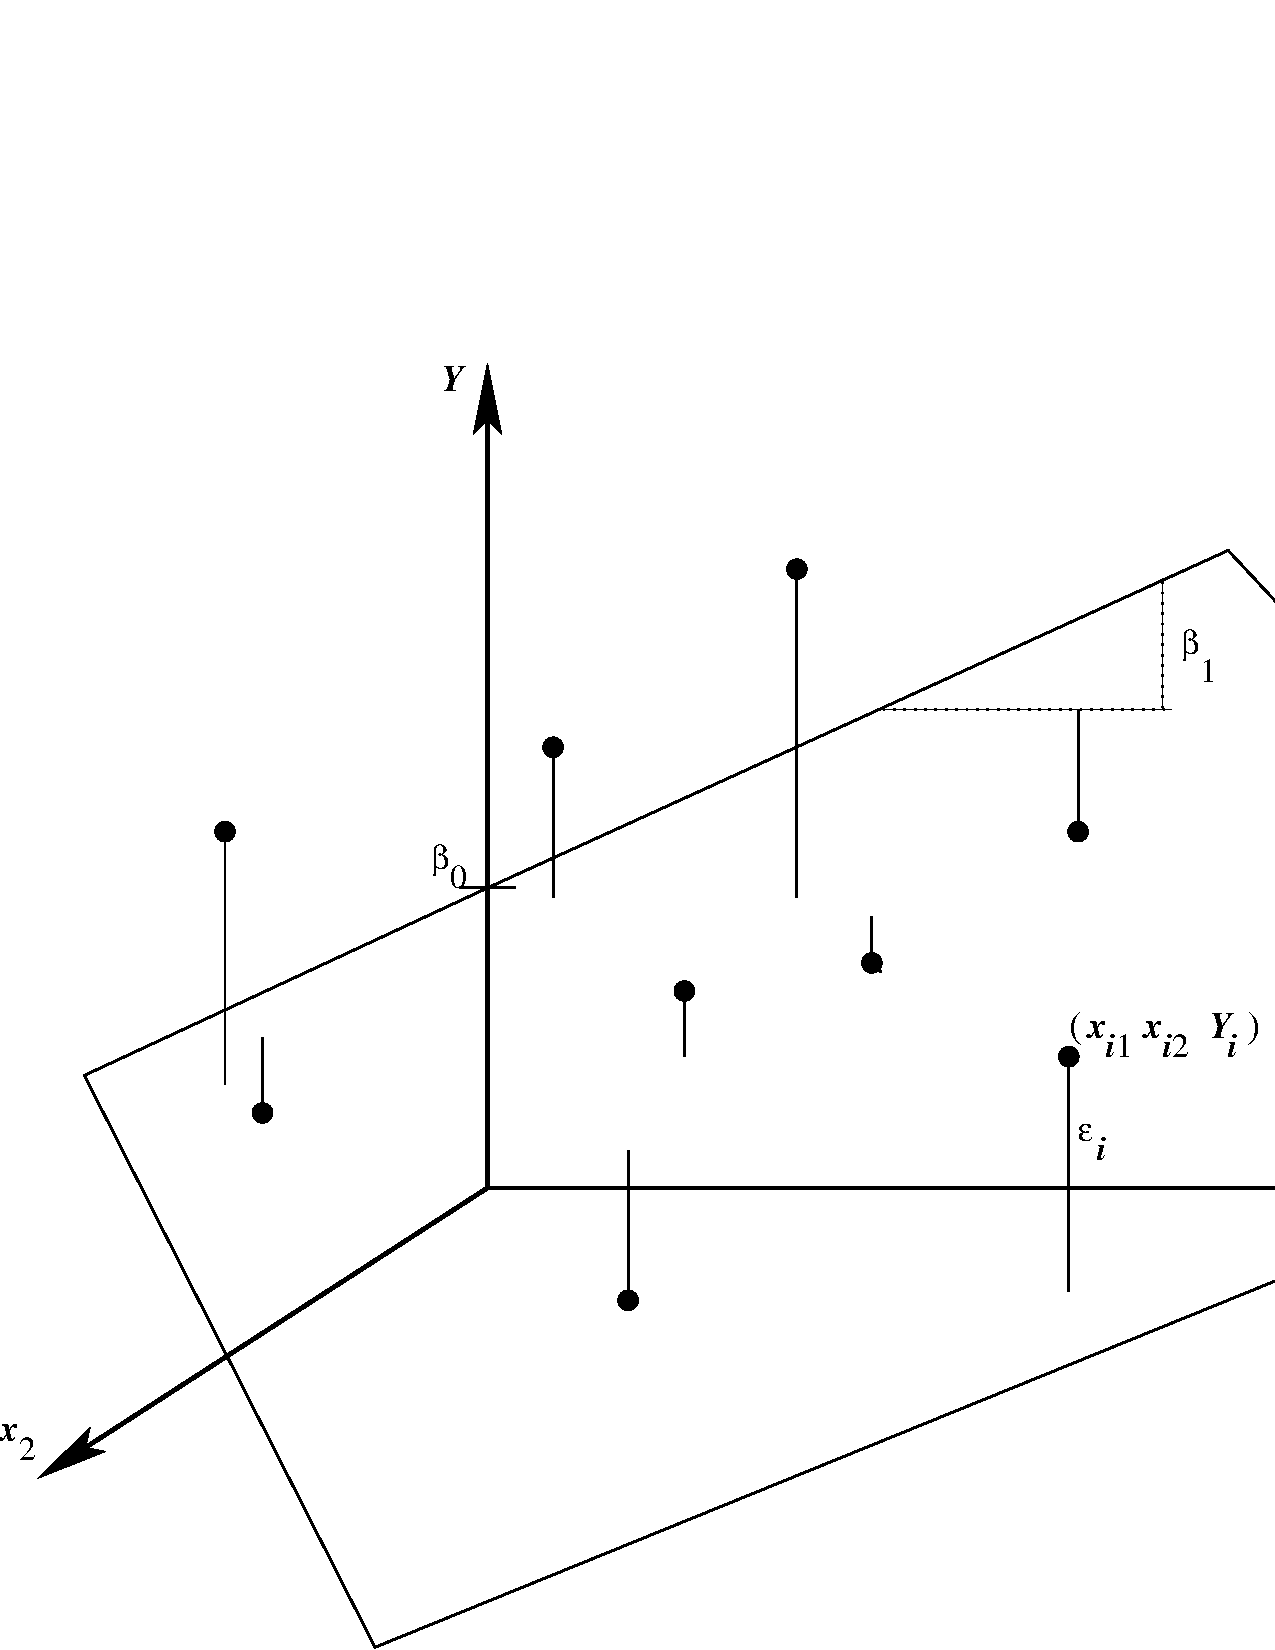
\includegraphics[scale=0.35, trim={0 0 0 5cm}]
{Chap5-AjusterRLM/Figures/reg_mult.pdf}}
\caption{Représentation géométrique du modèle de régression linéaire multiple.}\label{fig:rlm}
\end{figure}



\section{Estimation des coefficients}
\label{sec:EstimationParamètres}

%On présente ici de nouveau façons d'obtenir les estimateurs. Commenter sur la méthode du maximum de vraisemblance dans ce cas-ci; ça nous confirmerait qu'on a les meilleurs estimateurs possible. Noter également qu'on ne considère ici que les coefficients; on reviendra à l'estimation de la variance plus tard. }

\subsection{Méthode des moindres carrés}
\label{sec:EstimationRLMMoindresCarrés}


Comme dans le cas de la régression linéaire simple, on adopte à nouveau le principe des moindres carrés de Legendre. On cherche par conséquent le vecteur $\bobeta$ qui minimise la somme des carrés des résidus ($\sum_{i=1} ^n{\hat{\varepsilon}_i^2}$). Puisque le vecteur des résidus s'exprime
	\[ \hboeps= (\hat{\varepsilon}_1 , \hat{\varepsilon}_2, ... , \hat{\varepsilon}_n)' = \boY - \boX \hbobeta, \]
on a que
	\[\sum_{i=1}^n \hat{\varepsilon}_i^2= \hboeps' \hboeps= (\boY - \boX \hbobeta)' (\boY - \boX \bobeta)= f(\hbobeta)\]

En utilisant les propriétés des matrices (voir \ref{sec:prop_calc_mat}), $f(\hbobeta)$ s'écrit comme
\begin{eqnarray*}
	f(\hbobeta)&=&(\boY' - (\boX \hbobeta)')(\boY - \boX \hbobeta) \\
	&=& \boY' \boY - \boY' \boX \hbobeta - (\boX\hbobeta)' \boY + (\boX\hbobeta)' (\boX\hbobeta) \\
	&=& \boY' \boY - 2\hbobeta'\boX'\boY  + \hbobeta'\boX'  \boX\hbobeta
\end{eqnarray*}
Dans la dernière égalité on a utilisé le fait que $\boY'\boX\hbobeta=(\boX\hbobeta)'\boY=\hbobeta'\boX'\boY$, ce qu'on peut facilement démontrer puisque ces quantités sont des scalaires.

On obtient alors une fonction quadratique de $\hbobeta$. Pour minimiser $\sum_{i=1} ^n{\hat{\varepsilon}_i^2}$, on dérive $f(\hbobeta)$ par rapport à $\hbobeta$ et on pose $f'(\hbobeta)=0$ de la manière suivante :
\[
\begin{MAT}(r)[2pt,0pt,3cm]{c}
\frac{\partial f(\hbobeta)}{ \partial \hbobeta} \\
\end{MAT}
 = \left[
\begin{MAT}(r)[2pt,0pt,5.5cm]{c}
\frac{\partial f(\hbobeta)}{ \partial \hat{\beta}_0} \\
\frac{\partial f(\hbobeta)}{ \partial \hat{\beta}_1} \\
\vdots\\
\frac{\partial f(\hbobeta)}{ \partial \hat{\beta}_p} \\
\end{MAT}
\right] = \left[
\begin{MAT}(r)[2pt,0pt,5.5cm]{c}
0\\
0 \\
\vdots\\
0\\
\end{MAT}
\right]
\]
On obtient un système de $p+1$ équations à $p+1$ inconnues qu'il est possible d'exprimer sous format matriciel comme
	\[\frac{\partial f(\hbobeta)}{ \partial \hbobeta} = -2\boX' \boY + 2\boX' \boX \hbobeta =0\]

On veut donc résoudre $\boX' \boX \hbobeta = \boX' \boY$. Dans le cas où la matrice $\boX' \boX$ est inversible (de plein rang) on obtient que,
\begin{eqnarray}
	\underbrace{\hbobeta}_{(p+1)\times 1}=\underbrace{(\boX' \boX)^{-1}}_{(p+1)\times(p+1)} \underbrace{\boX'}_{(p+1)\times n} \underbrace{\boY}_{n\times 1}.
\label{eq:est_beta}
\end{eqnarray}

\begin{remarque}
La matrice $\boX' \boX$ n'est pas  inversible si le nombre d'observations $n$ est inférieur au nombre de paramètres à estimer $p'$, ou si une ligne de cette matrice est une combinaison linéaire des autres. Dans le premier cas, on pourra utiliser une méthode plus complexe, décrite à la section \ref{sub:lasso}. Dans le second cas, il faudra retirer cette variable du modèle. Voir aussi à cet effet le chapitre \ref{sec:Multicolinéarité} sur la multicolinéarité.
\end{remarque}


\subsubsection{Application au cas $p=1$}

Puisque le modèle de RLS est un cas particulier du modèle de RLM, il sera rassurant de vérifier que l'équation \ref{eq:est_beta} mène aux mêmes estimateurs que ceux de la section \ref{sec:AjusterRLS}.

Pour la RLS, la matrice d'incidence $\boX$ et sa transposée s'expriment comme :
\[
\begin{MAT}(r){c}
\boX\\
\end{MAT}
= \left[
\begin{MAT}(r){cc}
1 &  x_1\\
1 & x_2 \\
\vdots & \vdots  \\
1 & x_n \\
\end{MAT}
 \right]
\begin{MAT}(r){c}
\boX' \\
\end{MAT}
= \left[
\begin{MAT}(r){ccc}
1 & \ldots & 1\\
x_1 & \cdots & x_n \\
\end{MAT}
\right]
\]

On commence par calculer $\boX' \boX$.
\[
\begin{MAT}(e){c}
\boX' \boX\\
\end{MAT}
 = \left[
\begin{MAT}(e)[2pt,0pt,3cm]{cc}
n &  \sum_{i=1}^n x_i  \\
\sum_{i=1}^n x_i & \sum_{i=1}^n x_i^2 \\
\end{MAT}
\right] = \left[
\begin{MAT}(e)[2pt,0pt,3cm]{cc}
n & n\overline{x}\\
n\overline{x} & \sum_{i=1}^n x_i^2 \\
\end{MAT}
\right]
\]

Puis on trouve son inverse en se basant sur la formule d'inversion d'une matrice de dimension $2\times 2$. La première étape consiste à calculer le déterminant
$$	\mbox{det}(\boX'\boX) = n \sum_{i=1}^n x_i^2 - n^2\overline{x}^2
	= n \left(\sum_{i=1}^n x_i^2 - \sum_{i=1}^n \overline{x}^2\right)
	= n \sum_{i=1}^n  (x_i^2 - \overline{x}^2)
	= n \sum_{i=1}^n  (x_i - \overline{x})^2
	= n S_{xx}
$$

On a donc
\[
\begin{MAT}{c}
(\boX' \boX) ^{-1}\\
\end{MAT}
 =
\begin{MAT}{c}
\frac{1}{nS_{xx}}\\
\end{MAT}
\left[
\begin{MAT}(e){cc}
\sum_{i=1}^n x_i^2 & -n\overline{x}\\
-n\overline{x} & n \\
\end{MAT}
\right]
\]

On peut ensuite calculer $\hbobeta= (\boX' \boX)^{-1} \boX' \boY$.
\begin{align*}
\begin{MAT}{c}
\hbobeta \\
\end{MAT}
&= \frac{1}{nS_{xx}} \left[
\begin{MAT}{cc}
\sum_{i=1}^n x_i^2 & -n\overline{x}\\
-n\overline{x} & n \\
\end{MAT}
\right] \left( \left[
\begin{MAT}{cccc}
1 & 1 & \ldots &1 \\
x_1 & x_2 & \cdots & x_n\\
\end{MAT}
\right] \left[
\begin{MAT}{c}
Y_1 \\
Y_2 \\
\vdots \\
Y_n \\
\end{MAT}
\right] \right) \\
%
&
= \frac{1}{nS_{xx}} \left[
\begin{MAT}{cc}
\sum_{i=1}^n x_i^2 & -n\overline{x}\\
-n\overline{x} & n \\
\end{MAT}
\right] \left[
\begin{MAT}{c}
\sum_{i=1}^n Y_i \\
\sum_{i=1}^n x_i Y_i \\
\end{MAT}
\right]\\
%
& = \frac{1}{nS_{xx}} \left[
\begin{MAT}{c}
\sum_{i=1}^n x_i^2 n\overline{Y} - \sum_{i=1}^n x_i Y_i n\overline{x} \\
-\sum_{i=1}^n Y_i n\overline{x} + n \sum_{i=1}^n x_i Y_i\\
\end{MAT}
\right]
\end{align*}

On obtient donc
\begin{eqnarray*}
	\hat{\beta}_1 &=& \frac{n \sum_{i=1}^n x_i Y_i - n^2\overline{x} \overline{Y}}{n S_{xx}}= \frac{S_{xy}}{S_{xx}}.
\end{eqnarray*}

Pour l'ordonnée à l'origine, on a
\begin{eqnarray*}
	\hat{\beta}_0 &=& \frac{n \overline{Y} \sum_{i=1}^n x_i^2 - n\overline{x} \sum_{i=1}^n x_i Y_i}{nS_{xx}}
\end{eqnarray*}
En ajoutant $n\overline{x}^2\overline{Y} -n\overline{x}^2\overline{Y}$ au numérateur, on obtient que
\begin{eqnarray*}
		\hat{\beta}_0 & = & \frac{\overline Y(\sum x_i^2-n\overline x^2)-\overline x(\sum x_i Y_i-n\overline x\overline Y)}{S_{xx}} \\
       &=& \frac{\overline{Y}S_{xx} - \overline{x}S_{xy}}{S_{xx}} \\
	&=& \overline{Y} - \overline{x} \hat{\beta}_1 .
\end{eqnarray*}
On obtient donc exactement les mêmes résultats qu'en \eqref{eq:dbeta0egal0}.  et \eqref{eq:beta1}.

\begin{remarque}
De façon plus générale, en RLM,
\begin{eqnarray*}
	\hat{\beta}_0 &=& \overline{Y} - \overline{x}'_* \hat{\beta}_*\\
	&=& \overline{Y} - \sum_{i=1}^p \hat{\beta}_i \overline{x}^*_i
\end{eqnarray*}
où $\hat{\beta}_*$ est le vecteur des coefficients amputé de $\hat{\beta}_0$ et $\overline{X}_*$ est le vecteur contenant la moyenne de chaque variable (sans la colonne de 1).
\end{remarque}


\subsection{Argument géométrique}
\label{sec:ArgumentGéométrique}

Voyons maintenant comment arriver à \ref{eq:est_beta} à l'aide d'un argument géométrique.

Dans le modèle de régression linéaire multiple, on cherche à écrire $\boY$ comme une combinaison linéaire des colonnes de $\boX$, plus une erreur $\boeps$. Autrement dit, on veut projeter $\boY$ dans le sous-espace vectoriel engendré par $\boX$. Si $\boX$ est de plein rang (inversible), cet espace aura $p'=p+1$ dimensions.

On appelle matrice chapeau la matrice de projection de $\boY$ dans l'espace de $\boX$, et on la dénote $\boH$ (voir la section \ref{sec:MatriceChapeau} pour plus de détails sur cette matrice). Le vecteur résiduel défini par $\hboeps = \boY-\hY = (\boI_n-\boH)\boY$ est alors perpendiculaire à l'espace engendré par $\boX$. La figure \ref{fig:geometrie} représente géométriquement le cas à 3 observations $\boY=(Y_1,Y_2,Y_3)$ où l'on a deux paramètres à estimer ($p'=2$).

\begin{figure}[htb!]
	\centering
		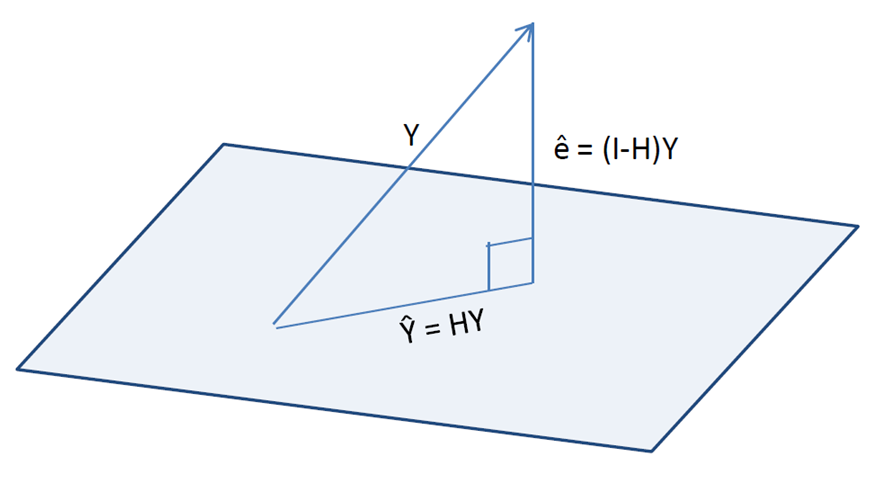
\includegraphics[scale = 0.9]{Chap5-AjusterRLM/Figures/geometrie}
	\caption{Représentation géométrique de la régression dans le cas où il y a deux paramètres à estimer.}
	\label{fig:geometrie}
\end{figure}

%Si $\boX$ n'est pas de plein rang, certaines colonnes de $\boX$ (certaines variables) sont linéairement dépendantes. Dans ce cas, il suffit de retirer une ou plusieurs variables.

Le vecteur des résidus est la projection de $\boY$ dans l'espace perpendiculaire à $\boX$. Toujours en considérant $\boX$ de plein rang, cet espace est de dimension $(n-p')$.

L'angle droit entre le vecteur des valeurs prédites ($\hY$) et le vecteur des résidus $\hboeps$ découle du fait que l'on ait choisi $\hbobeta$ de façon à minimiser la somme des résidus au carré, c'est-à-dire $\hboeps'\hboeps$. L'orthogonalité de $\hY$ et $\hboeps$ revient à dire que $\cov[\hboeps, \hY] = 0$. En effet, des vecteurs orthogonaux sont des vecteurs non corrélés. Dans le cas gaussien, ceci implique de plus que ces vecteurs sont indépendants.


Cette approche permet de refaire le calcul nous ayant mené \`a la formule pour $\hbobeta$. En effet, les résidus sont perpendiculaires au plan, car on souhaite faire une projection orthogonale. On peut donc dire qu'ils sont orthogonaux aux combinaisons linéaires des colonnes de $\boX$, en particulier à $\boX$ lui-même. Pour trouver la valeur de $\hbobeta$ telle
que $\boX$ est orthogonal \`a $\hboeps$, on doit résoudre
\begin{equation}\label{eqnorm:geo}
\boX'\hboeps=\boX'(\boY-\boX\hbobeta)=\bo{0}.
\end{equation}


On arrive donc tel que prévu à
$$\hbobeta=(\boX'\boX)^{-1}\boX'\boY.$$

\subsection{Méthode du maximum de vraisemblance}
\label{sec:RLM-MLE}

Comme pour la RLS, l'estimateur en \ref{eq:est_beta} peut être obtenu à l'aide de la méthode du maximum de vraisemblance. Nous omettons les détails ici.

La méthode du maximum de vraisemblance permet également d'estimer $\sigma^2$. Comme pour la RLS, l'estimateur du maximum de vraisemblance pour la variance des erreurs est toutefois biaisé. Nous utiliserons plutôt un estimateur non-biaisé de cette variance, lequel est dérivé à la section
\ref{sec:RLM-sigma}.

\newpage

\section{Exemple}

Cet exemple est tiré de \citet[][Exemple 14.1]{Hin_Mon_Gol_Bor:12}.
%\citet{Rag_Ber:01} exposent une analyse consistant à trouver un modèle de prévision des meurtrissures des pommes durant le tri et l'emballage.
Des expériences en laboratoire ont montré que le diamètre des meurtrissures (en mm) peut être expliqué en fonction de la hauteur de chute (en mm) et de la masse volumique des fruits (en g/cm$^3$). Le Tableau \ref{exp_data} présente des données typiques de ce type d'expérience.


\begin{table}[htb!]
\caption{Données pour l'exemple des meurtrissures de pêches}
\label{exp_data}
\begin{tabular}{|c|c|c|c|} \hline
numéro &  diamètre des meurtrissures  & hauteur de chute  & masse volumique  \\
 & [mm] & [mm] & [g/cm$^3$] \\
        & $Y_i$        & $x_{i1}$      &  $x_{i2}$ \\ \hline
 1   &   3,62  &   303,7  & 0,90      \\
 2   &   7,27  &   366,7  & 1,04     \\
 3   &   2,66  &  336,8   & 1,01     \\
 4   &   1,53  &  304,5   & 0,95      \\
 5   &   4,91  &  346,8   & 0,98      \\
 6   &   10,36 &   600,0    & 1,04       \\
 7   &   5,26  &   369,0    & 0,96       \\
 8   &   6,09  &   418,0    & 1,00           \\
 9   &   6,57  &   269,0    & 1,01        \\
 10  &   4,24  &   323,0    & 0,94         \\
 11  &   8,04  &   562,2  & 1,01          \\
 12  &   3,46  &   284,2  & 0,97           \\
 13  &   8,50   &   558,6  & 1,03           \\
 14  &   9,34  &   415,0    & 1,01            \\
 15  &   5,55  &   349,5  & 1,04            \\
 16  &   8,11  &   462,8  & 1,02            \\
 17  &   7,32  &   333,1  & 1,05            \\
 18  &   12,58 &   502,1  & 1,10            \\
 19  &   0,15  &   311,4  & 0,91            \\
 20  &   5,23  &   351,4  & 0,96            \\   \hline
\end{tabular}

\end{table}


Le modèle de régression linéaire multiple s'exprime sous forme matricielle comme


$$
\underbrace{\left(
\begin{array}{c}
3,62  \\
7,27  \\
2,66 \\
1,53 \\
\vdots \\
5,23  \\
\end{array} \right)}_{20\times 1}
 =  \underbrace{\left(\begin{array}{ccc}
            1	&      303,7  & 0,9     \\
            1	&      366,7  & 1,04    \\
            1 &         336,8 & 1,01 \\
            1 &           304,5 & 0,95 \\
            \vdots & \vdots & \vdots   \\
            1	&      351,4  & 0,96
\end{array}\right)}_{20\times 3}
\underbrace{\left(\begin{array}{c}
\beta_0 \\
\beta_1 \\
\beta_2
\end{array} \right)}_{3\times 1}+
\underbrace{\left(\begin{array}{c}
\varepsilon_1 \\
\varepsilon_2 \\
\varepsilon_3 \\
\varepsilon_4 \\
\vdots \\
\varepsilon_{20}
 \end{array}
 \right)}_{20\times 1}
 $$


Selon l'équation \ref{eq:est_beta}, on sait que $\hbobeta=(\boX'\boX)^{-1}\boX' \boY$.

La matrice $\boX'\boX$ est
\begin{eqnarray*}
\boX'\boX & = & \left(
\begin{array}{cccc}
1 & 1 & \cdots & 1 \\
303,7 & 366,7 & \cdots & 351,4 \\
0,90 & 1,04 & \cdots & 0,96
\end{array}
\right)
\left(
\begin{array}{ccc}
1 & 303,7 & 0,90 \\
1 & 366,7 & 1,04 \\
\vdots & \vdots & \vdots \\
1 & 351,4 & 0,96
\end{array}
\right) \\
& = & \left(
\begin{array}{ccc}
20 & 7767,8 & 19,33 \\
7767,8 & 3201646 & 7791,878 \\
19,93 & 7791,878 & 19,9077
\end{array}
\right).
\end{eqnarray*}
Le vecteur $\boX'\boY$ s'exprime comme
\begin{eqnarray*}
\left(
\begin{array}{cccc}
1 & 1 & \cdots & 1 \\
303,7 & 366,7 & \cdots & 351,4 \\
0,90 & 1,04 & \cdots & 0,96
\end{array}
\right)
\left(
\begin{array}{c}
3,62 \\
7,27 \\
\vdots \\
5,23
\end{array}
\right)
=
\left(
\begin{array}{r}
120,79 \\
51129,17 \\
122,70
\end{array}
\right).
\end{eqnarray*}
On en déduit donc que
\begin{eqnarray*}
\left(
\begin{array}{c}
\hat\beta_0 \\
\hat\beta_1 \\
\hat\beta_2
\end{array}
\right)
& = &
\left(
\begin{array}{ccc}
20 & 7767,8 & 19,33 \\
7767,8 & 3201646 & 7791,878 \\
19,93 & 7791,878 & 19,9077
\end{array}
\right)^{-1}
\left(
\begin{array}{r}
120,79 \\
51129,17 \\
122,70
\end{array}
\right) \\
& = &
\left(
\begin{array}{rrr}
24,63666 & 0,005321 & -26,74679 \\
0,005321 & 0,0000077 & -0,008353 \\
-26,74679 & -0,008353 & 30,096389
\end{array}
\right)
\left(
\begin{array}{r}
120,79 \\
51129,17 \\
122,70
\end{array}
\right) \\
& = &
\left(
\begin{array}{r}
-33,8310 \\
0,0134 \\
34,8900
\end{array}
\right)
\end{eqnarray*}
Par conséquent, le modèle de régression ajusté s'écrit comme
$$\hat Y=-33,831+0,0134x_1+34,890x_2.$$
L'espérance du diamètre moyen des meurtrissures d'une pêche de masse volumique nulle lancée d'une hauteur nulle (très hypothétique comme valeur!) est de $-33,831$ mm. L'augmentation d'un mm de la hauteur de la chute est associée à une augmentation attendue de 0,0134 mm du diamètre moyen des meurtrissures, pour une masse volumique constante. De même, l'augmentation d'un $g/cm^3$ de la masse volumique d'une pêche est associée à une augmentation attendue de $34,890$ mm du diamètre moyen des meurtrissures, pour une hauteur de chute constante.


